\chapter{Описание робота}
\section{Общие сведения}
Робот Robotino был создан и выпускался немецкой компанией Festo Didactic для применения в образовательных целях.
Всего компанией производителем было разработано три версии (или поколения) этого робота: Robotino~1.0, Robotino~2.0 и Robotino~3.0\lefteqn{.}\footnote{То, что данный робот существует в трех версиях, следует, например, из~\cite{history_hard_page}, а также из того, что на сайте производителя существуют страницы, посвященные двум последним версиям робота (см.~\cite{festo_page_with_robotino_until_2013, festo_page_with_robotino_3}) и на первой из них есть упоминание об еще более старой версии данного робота.}
Данное руководство посвящено описанию роботов второй(-го) из них.

Внешний вид робота Robotino~2.0 показан на рисунке~\ref{img_gen_view_of_robotino}.
Большинство из отмеченных на нем частей робота будут подробно описаны ниже по тексту.
О~датчике касания~3, о котором далее не последует отдельного повествования, достаточно отметить лишь то, что он, выполняющий также защитные функции, работает как концевой выключатель, сигнализируя только о факте собственного контакта с внешними объектами.

\begin{figure}[h]
	\centering
	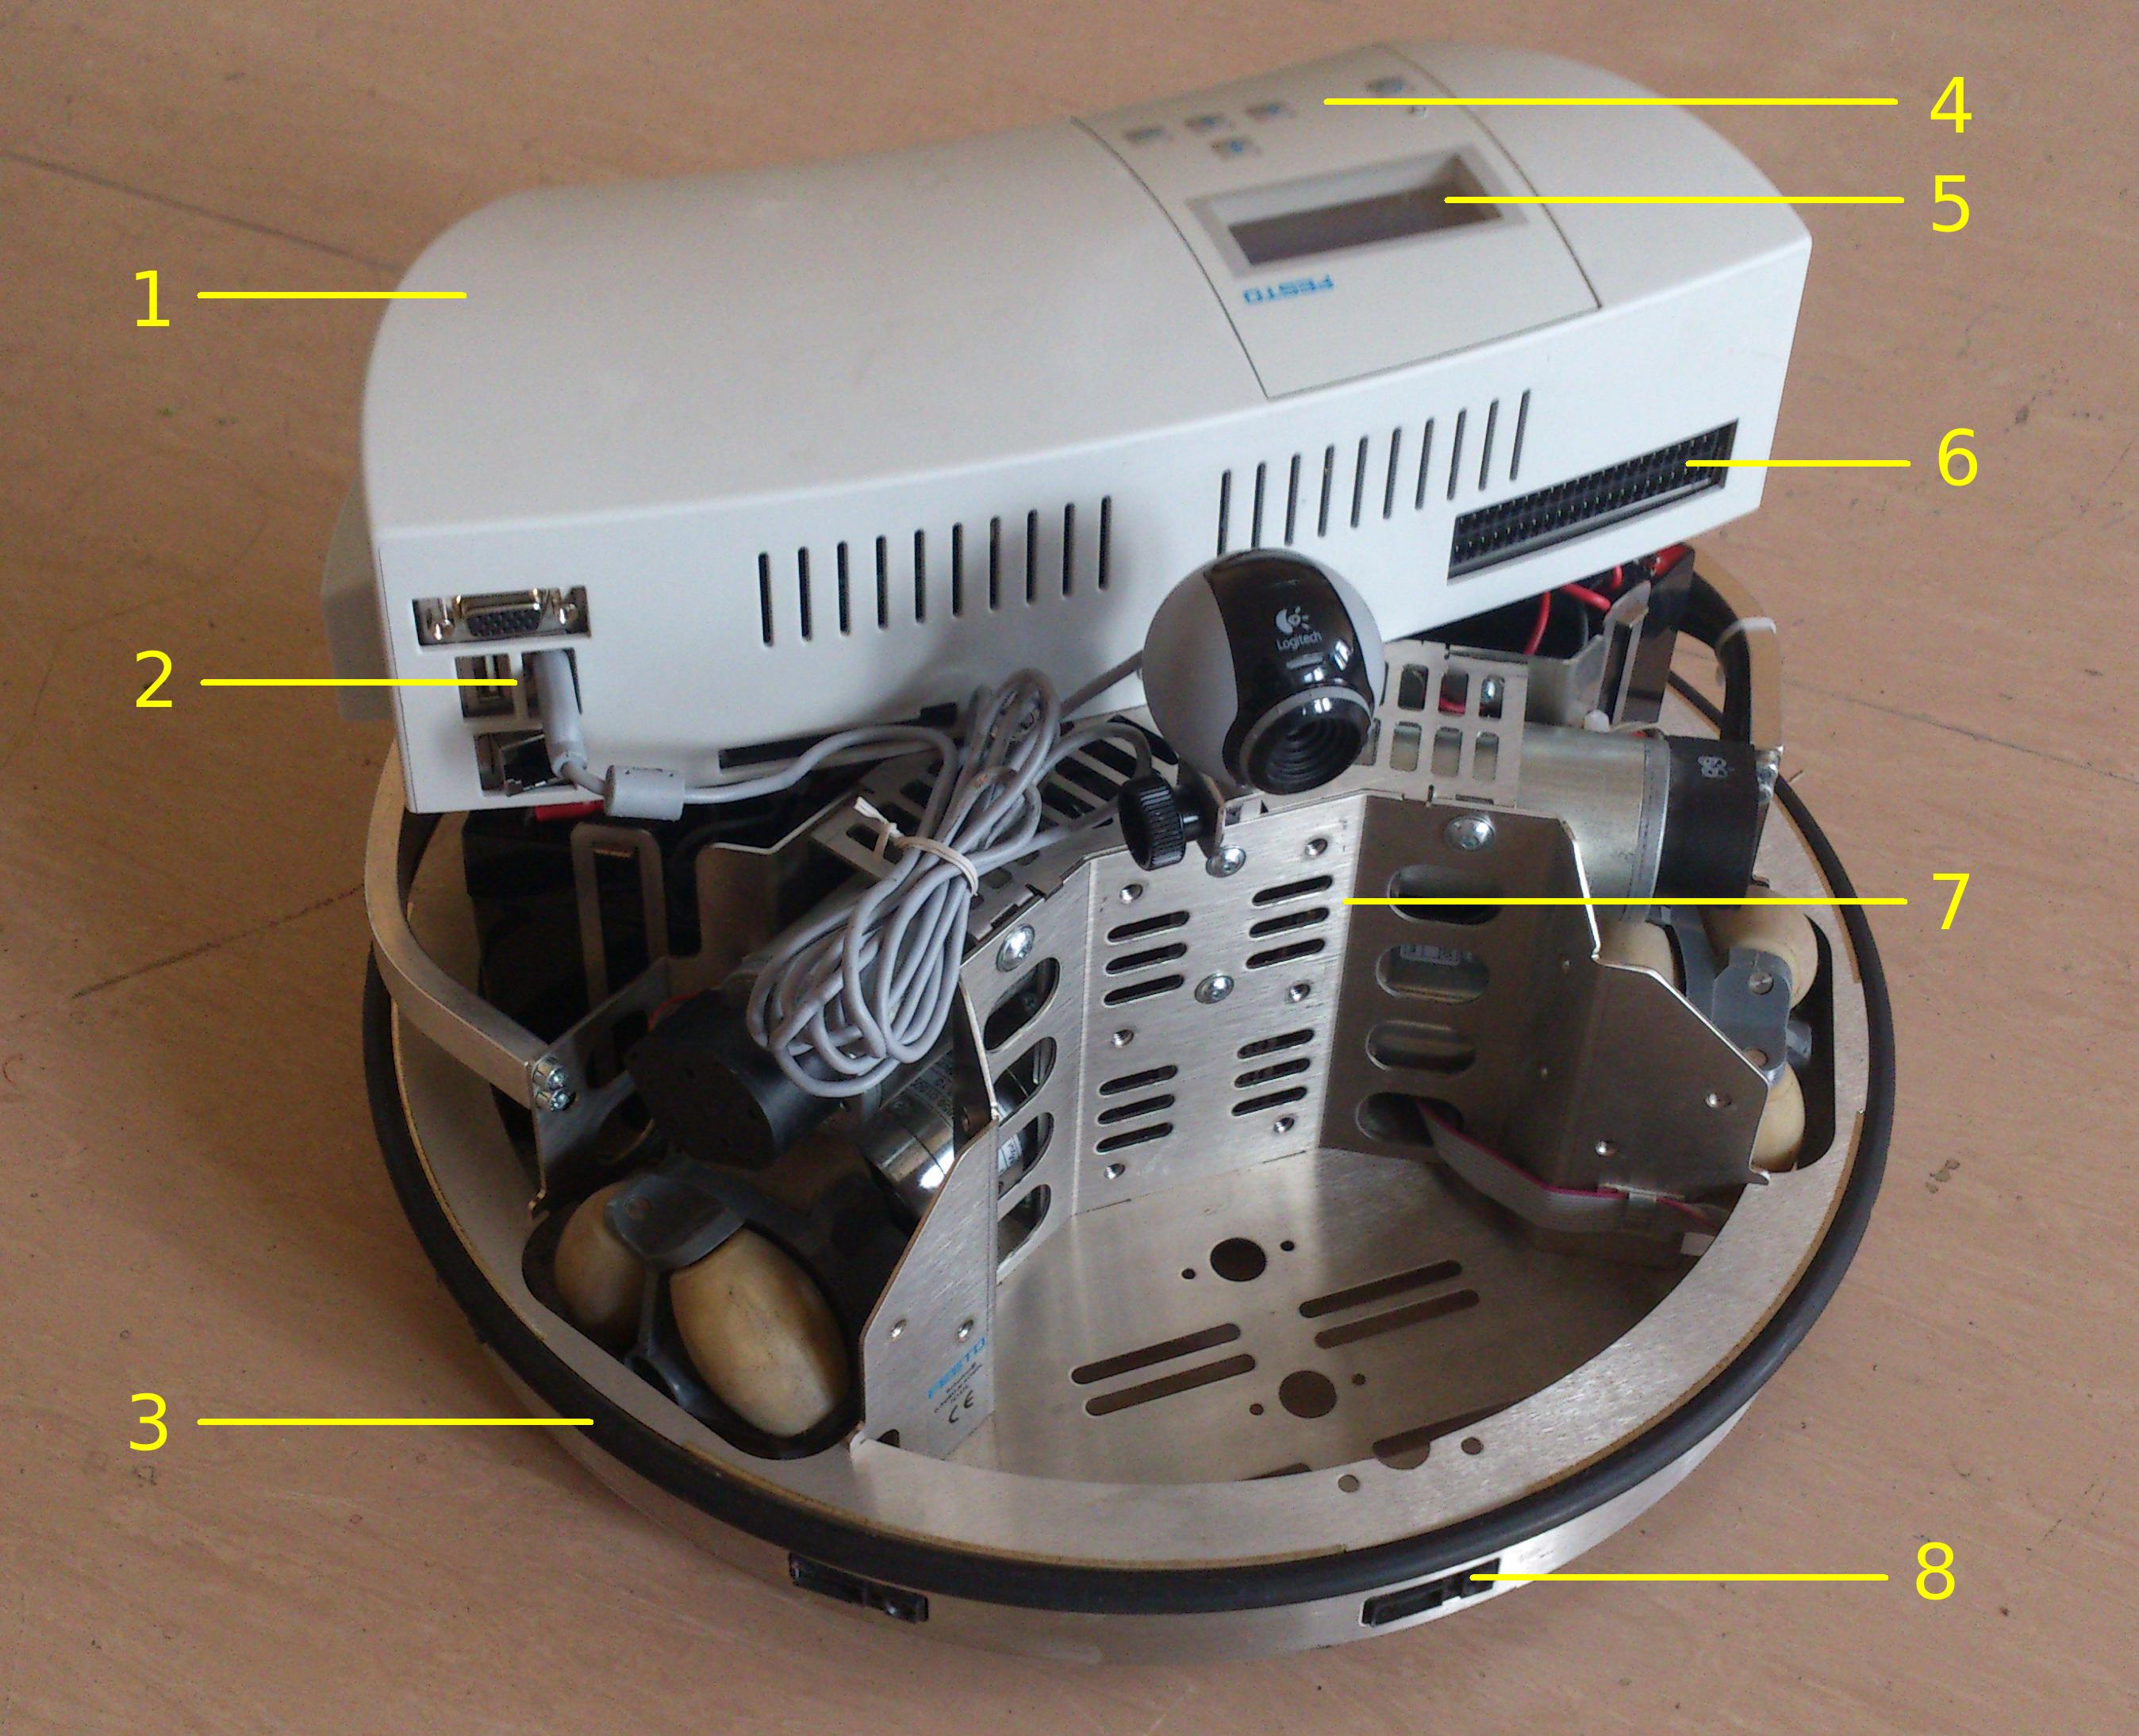
\includegraphics[height = 7cm]{robotino_gen_view.jpg}
	\caption{Робот Robotino: 1~--- блок с бортовым компьютером и управляющей электроникой; 2~--- разъемы VGA~\texttimes{}~1, USB~2.0~\texttimes{}~2 и Ethernet~\texttimes{}~1; 3~--- датчик касания; 4, 5~--- кнопочно-дисплейный интерфейс; 6~--- порты питания и ввода-вывода; 7~--- шасси; 8~--- оптический дальномер.}
	\label{img_gen_view_of_robotino}
\end{figure}



\section{Ходовая часть робота}
Ходовая часть данного робота (см.~рисунок~\ref{img_robotinos_chassis}) снабжена тремя всенаправленными колесами~4, каждое из которых приводится в движение отдельным двигателем~2 постоянного тока через ременную передачу~1 и редуктор (он находится под двигателем и на рисунке~\ref{img_robotinos_chassis} не виден).
Благодаря такому ее устройству Robotino может двигаться на плоскости совершенно произвольным образом.

\begin{figure}[h]
	\centering
	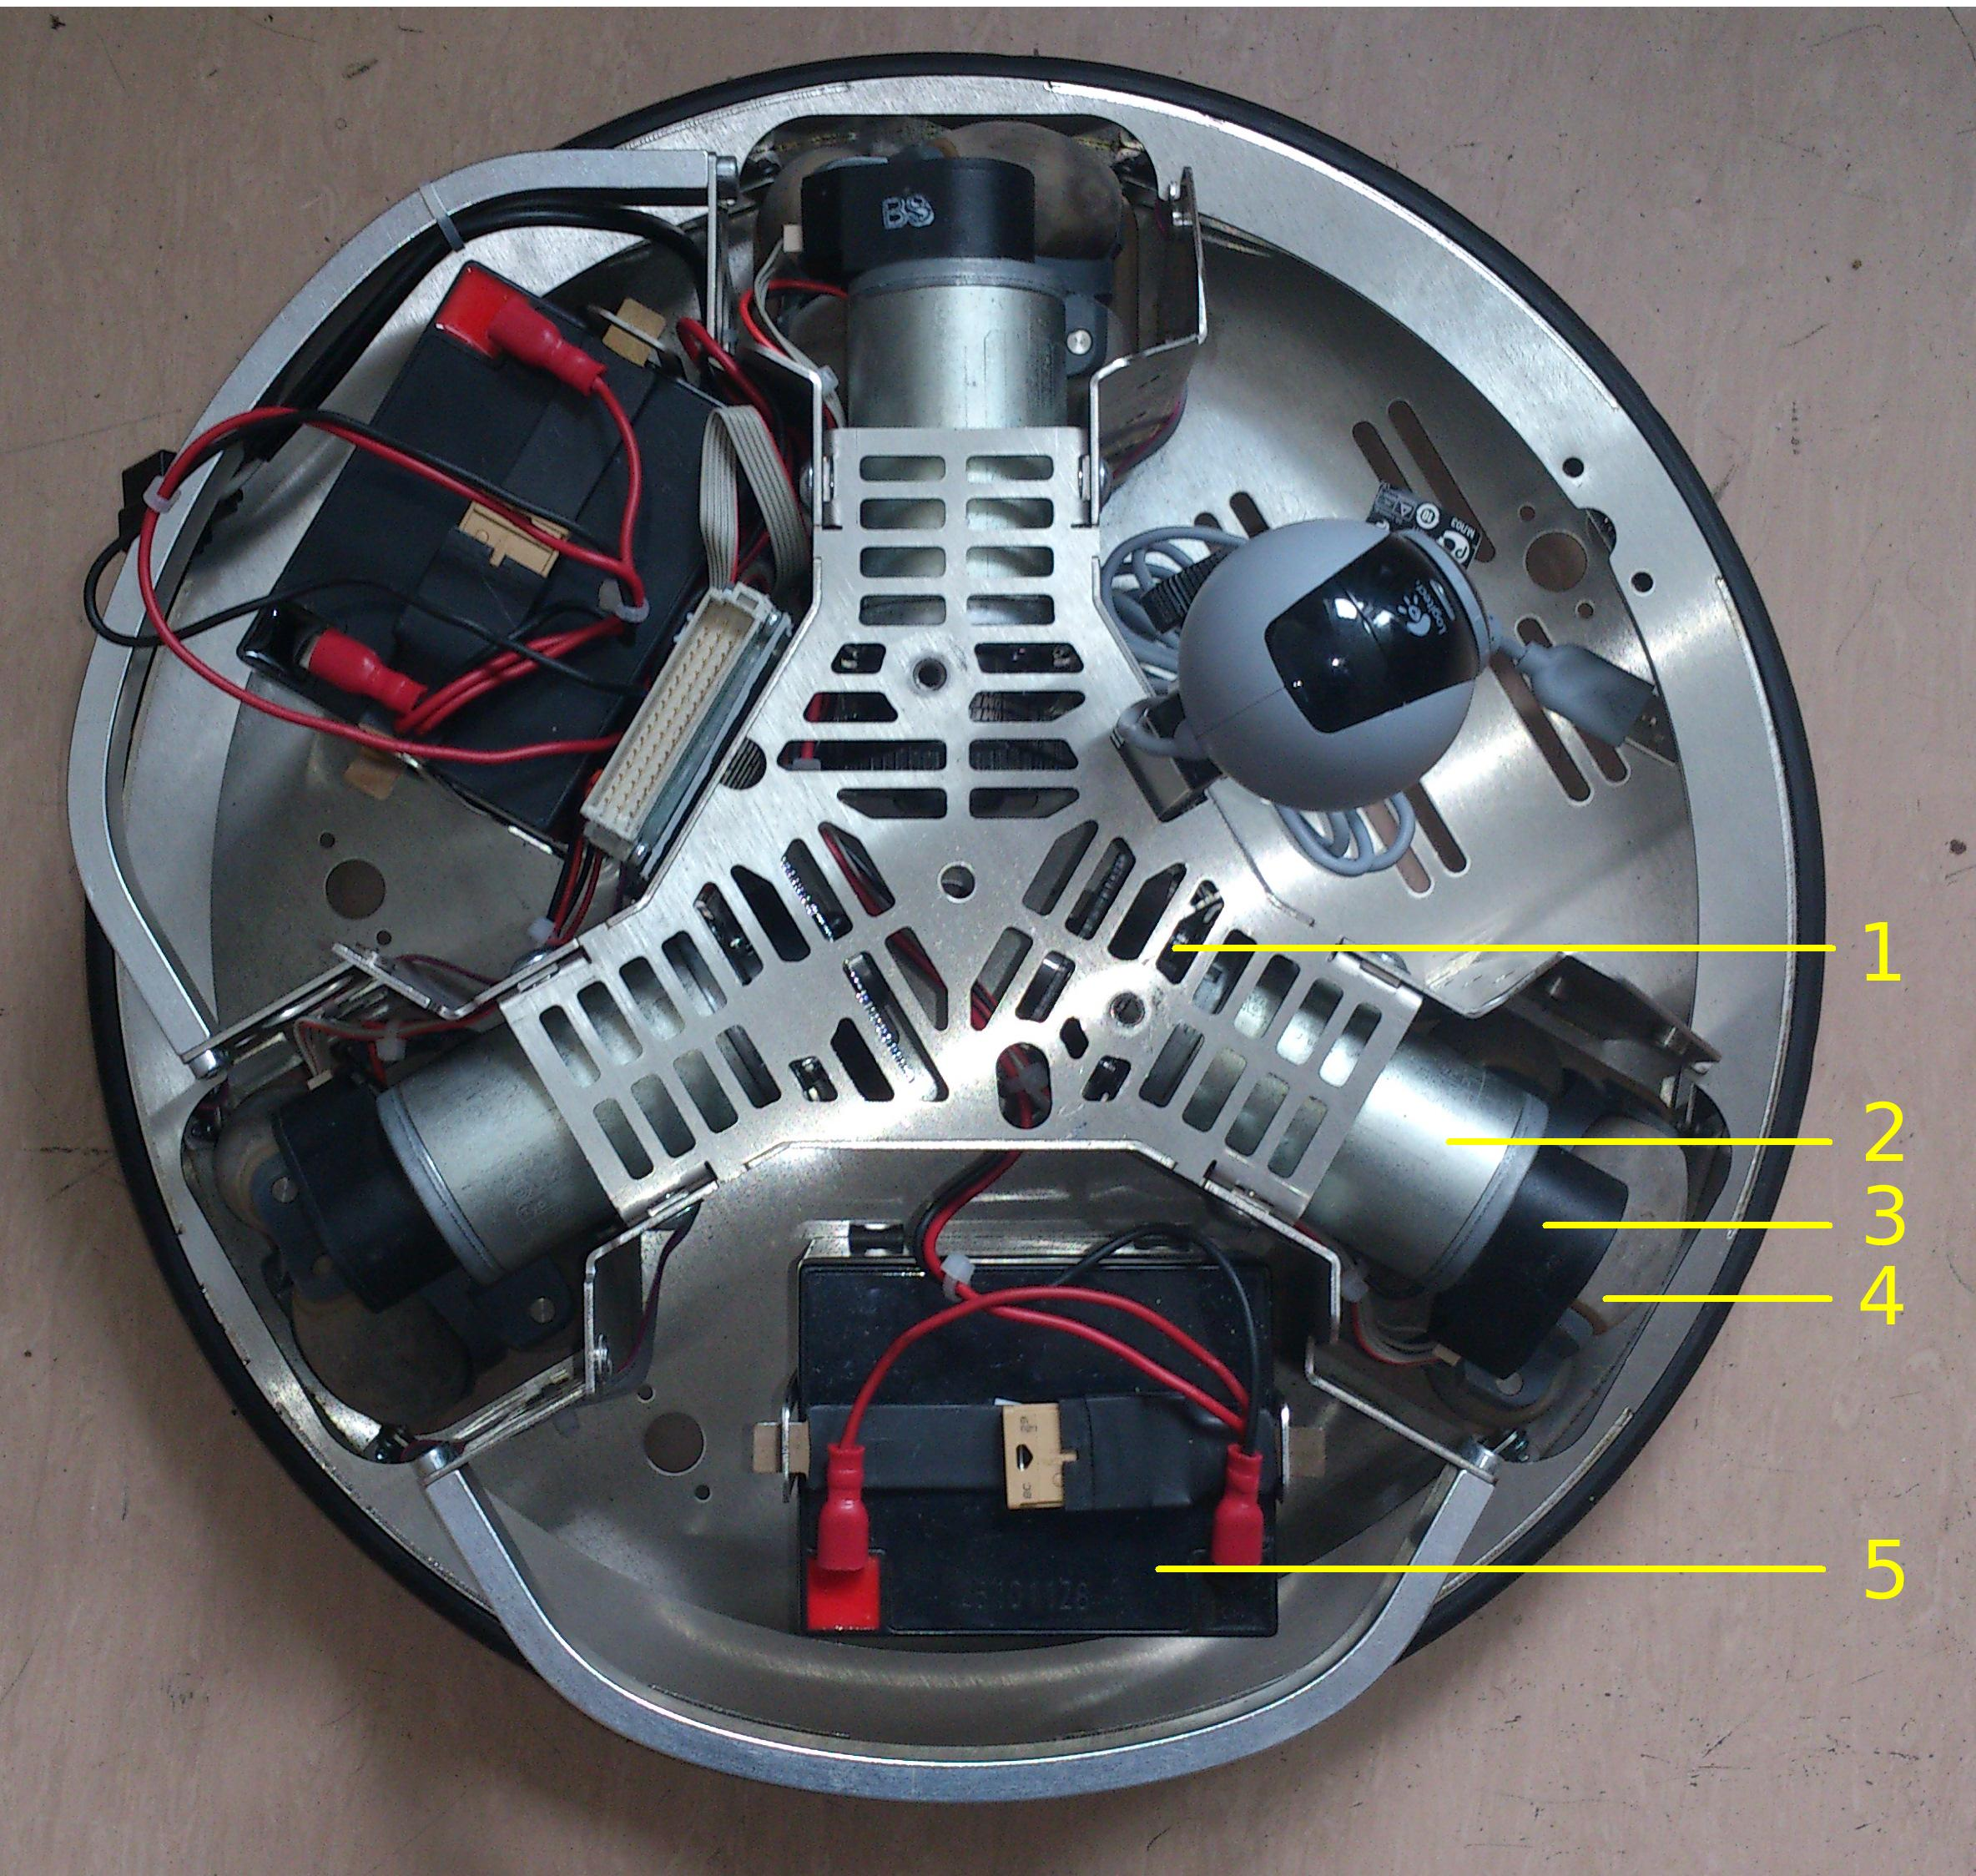
\includegraphics[height = 7cm]{robotino_chassi.jpg}
	\caption{Строение ходовой части робота: 1~--- передача с зубчатым ремнем; 2~--- двигатель постоянного тока; 3~--- энкодер; 4~--- всенаправленное колесо; 5~--- аккумулятор.}
	\label{img_robotinos_chassis}
\end{figure}

Максимальная скорость поступательного движения робота согласно~\cite{festo_page_with_robotino_until_2013} равна~10~км/ч.



\section{Бортовые компьютер и электроника}
Командный блок (<<голова>>) робота содержит компьютер, на котором установлен Linux Ubuntu 9.04, и иную электронику, необходимую для работы с датчиками, двигателями и проч.
Информация о них может быть найдена в~\cite{history_hard_page, festo_page_with_robotino_until_2013, main_manual}, при этом автор не берется комментировать ее достоверность.

В~заключение остается добавить, что на кафедральных роботах их родные роутеры заменены на маршрутизаторы TL-WR702N.



\section{Порты питания и линии ввода-вывода}
Входы-выходы~6 (см.~рисунок~\ref{img_gen_view_of_robotino}, а также рисунки из~\cite[стр.~74]{main_manual} и~\cite{docs_page_analog}) нужны для подключения к роботу дополнительного оборудования.
Они включают в себя
\begin{itemize}
    \item 8 аналоговых входов (AIN0--AIN7),
    \item 8 цифровых входов (DI0--DI7),
    \item 8 цифровых выходов (DO0--DO7),
    \item 2 набора портов релейного переключения (REL0\_* и REL1\_*),
    \item 10 выходов питания (24V и GND)
\end{itemize}
и предназначены для работы со следующими электрическими сигналами:
\begin{itemize}
    \item допустимое напряжение для подачи на аналоговые входы~--- от 0 до +10~В~\cite[стр.~74]{main_manual},~\cite{docs_page_analog};
    \item при выставлении на какой-либо цифровой выход логического нуля (<<false>> в соответствующей функции) потенциал на нем относительно земли будет равен 0~В, при выставлении логической~<<1>> (<<true>> в соответствующей функции)~--- +10~В~\cite{docs_page_digit_out}\footnote{Измерение мультиметром, однако, во втором случае показывает значение, близкое к +24~В.};
    \item при подаче на какой-либо цифровой вход напряжения меньшего, чем 5.75~В, входной сигнал будет интерпретирован как логический~<<0>>, а при большего, чем 8.6~В~--- как логическая~<<1>>~\cite{docs_page_digit_in}\footnote{О~допустимых верхней и нижней границах информации в сети найти не удалось. Принимая во внимание сказанное в~\cite{docs_page_digit_out} о цифровых выходах можно предположить, что максимально большое из допустимых напряжений имеет значение, равное~+10~В.}.
    \item информацию о максимально допустимом токе, который может быть обеспечен выходами питания, найти не удалось; можно лишь предполагать, что он не должен превышать 4.5~A~--- значения, которое указано в~\cite[стр.~58]{main_manual} и которое, к слову сказать, близко к значению, на которое рассчитаны предохранители робота (5~А).
\end{itemize}

Смысл портов релейного переключения установить не удалось.

Подключение проводных контактов устройств к рассмотренным портам ввода-вывода робота осуществляется с помощью специальных клеммников, пример которых можно видеть на рисунке~\ref{img_terminal}.
Для этого последние с закрепленными в них контактами устройств\footnote{Для закрепления провода в гнезде клеммника отожмите, например отверткой, соответствующий фиксатор так, как это показано на рисунке~\ref{img_terminal}.} попросту вставляются по одному в верхний и нижний ряд соответствующих отверстий (см.,~например, рисунок~\ref{img_inductive_connect}).

\begin{figure}[h]
	\centering
	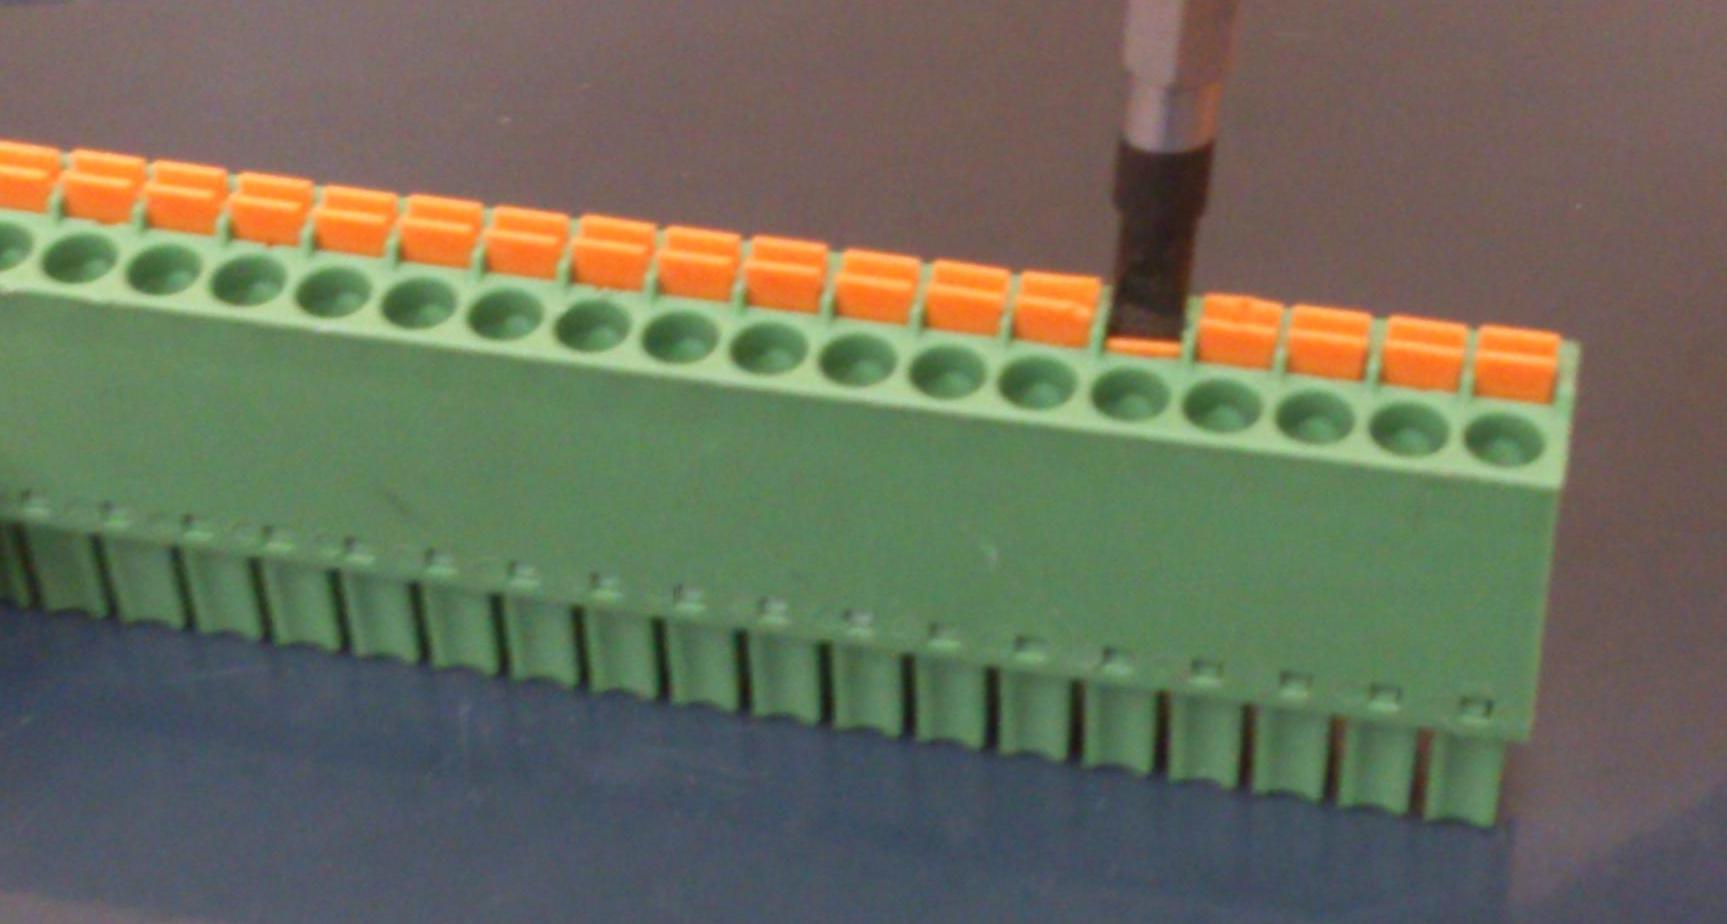
\includegraphics[height = 4cm]{terminal.jpg}
	\caption{Внешний вид клеммников Robotino.}
	\label{img_terminal}
\end{figure}



\section{Периферийные дальномеры}
Робот Robotino имеет 9 оптических дальномеров, внешний вид которых можно видеть на рисунке~\ref{img_gen_view_of_robotino}.
Каждый из них согласно \cite[стр.~68]{main_manual} рассчитан на измерение расстояний до объектов в пределах от 4 до 30~см.

Схема расположения дальномеров представлена на рисунке~\ref{img_scheme_of_rangerfinders_places}.
Красным и зеленым отрезками, на нем показаны оси $OX$ и $OY$ правосторонней системы координат, жестко связанной с роботом так, что положительное направление оси абсцисс совпадает с направлением <<взора>> робота.
Окружностью радиусом 48.5~см обозначена приблизительная граница области видимости датчиков.
Последнее значение получается, если к наибольшему расстоянию до препятствия, фиксируемому дальномерами, (30~см) прибавить радиус робота, равный 18.5~см~\cite{festo_page_with_robotino_until_2013}.

\begin{figure}[h]
	\centering
	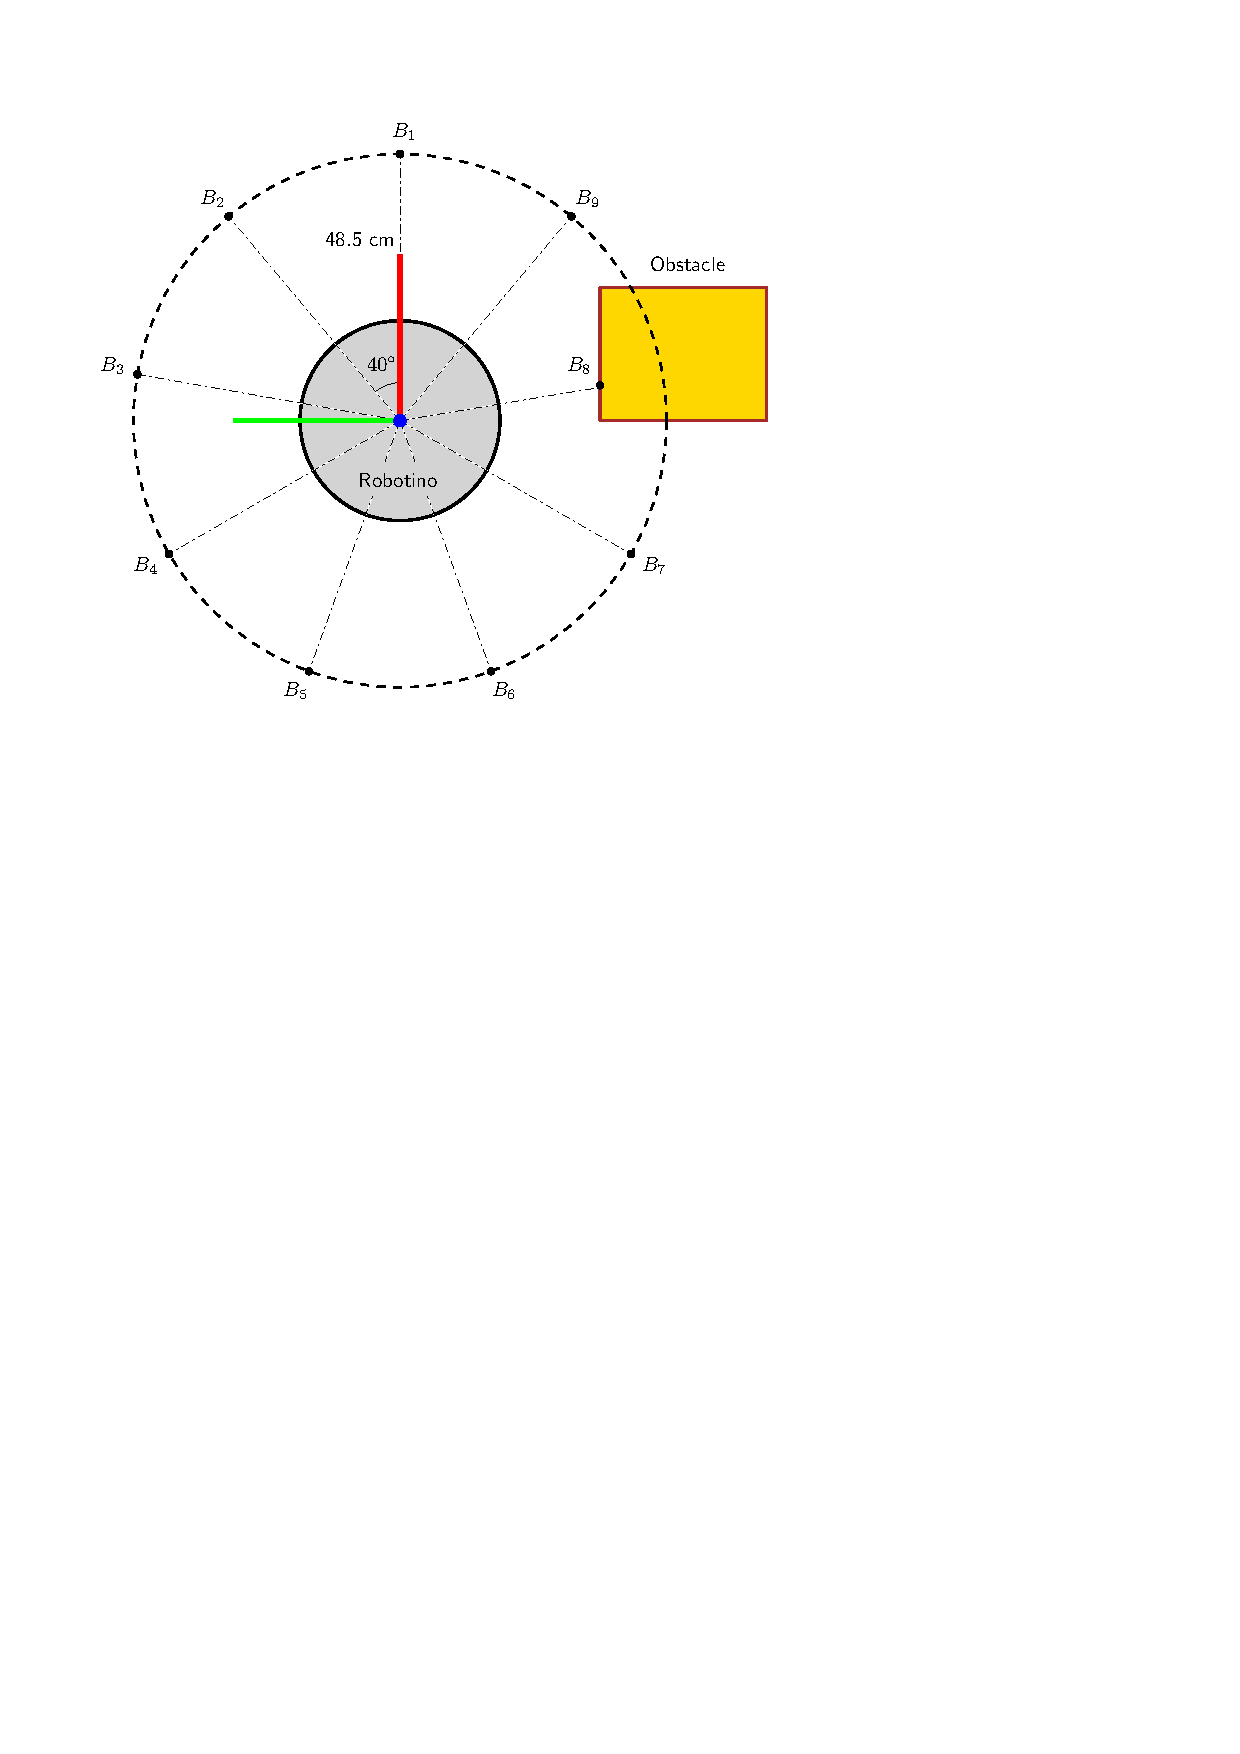
\includegraphics[width=0.6\textwidth]{scheme_of_rangerfinders_places.pdf}
	\caption{Схема расположения дальномеров на роботе Robotino.}
	\label{img_scheme_of_rangerfinders_places}
\end{figure}
